\chapter{IDEIA GERAL}
\label{conceituacaoEIdeiaGeral} %mudar label
Este capítulo tem como foco expôr o processo de desenvolvimento da nossa pesquisa, e o amadurecimento do tema abordado.

\section{Escolha do tema}
\label{sec: escolhaDoTema}
Durante as eleições de 2014, várias pesquisas foram levantadas em diversas redes sociais sobre a opinião das pessoas a respeito dos atuais candidatos. Analisando essas pesquisas, percebemos que muitas delas, apenas ao comparar o número de menções dos candidatos, não expunham a opinião expressa por trás dessas menções.

Percebemos então que pesquisas em áreas diversas apenas levavam em conta a quantidade de menções, e raramente consideravam se a opinião expressa da pessoa que a fez era positiva, negativa, ou neutra sobre o item mencionado.

Essa realidade nos motivou a desenvolver uma aplicação capaz de gerar uma pesquisa, levando em conta o contexto em que a palavra é encontrada. Tal pesquisa com essa característica poderia mostrar que um número alto de menções nas redes sociais não é garantia de aceitação popular.

No decorrer da pesquisa descobrimos o termo Análise de Sentimento(Seção \ref{sec: analiseSentimento}), que se ajustava com a ideia de analisar as opiniões embutidas nos textos coletados das redes sociais.

Pesquisando mais sobre o assunto, percebemos que o nível de complexidade poderia ser suficiente para dois trabalhos de graduação:
\begin{itemize}
    \item O primeiro sendo responsável por armazenar informações coletadas de redes sociais, de forma organizada e eficiente, em um banco de dados;
    \item O segundo, implementar uma ferramenta que realize a análise de sentimento na língua portuguesa, e aplicá-la nos textos armazenados usando o modelo do primeiro trabalho.
\end{itemize}

\section{Visão geral da aplicação}
\label{sec: visaoGeralDaAplicacao}
Escolhemos implementar o modelo de banco de dados nesse trabalho, já que a análise de sentimentos depende de informações previamente armazenadas.
Portanto, nossa aplicação deve:
\begin{enumerate}
    \item Receber um tema de pesquisa como entrada;
    \item Aplicar métodos de busca em diversas redes sociais;
    \item Armazenar os textos coletados em um banco de dados modelado especialmente para a aplicação da análise de sentimento.
\end{enumerate}

\begin{figure}[ht]
  \centering
  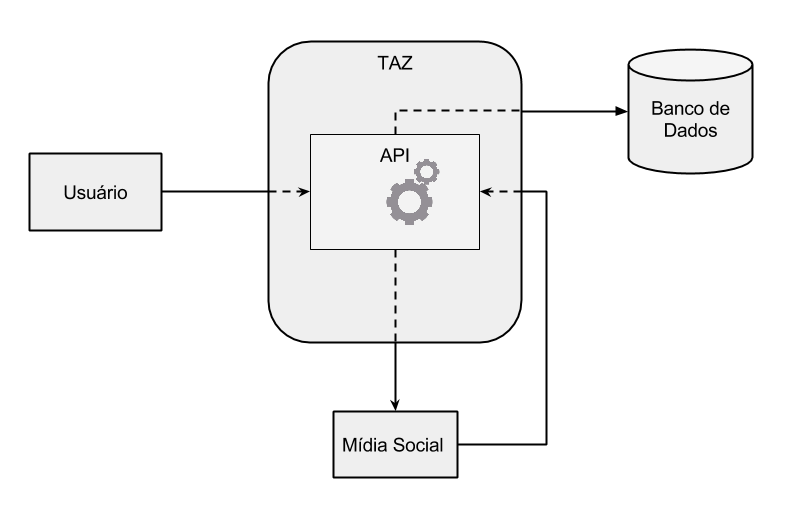
\includegraphics[width=.8\textwidth]{images/esquema}
 
  \caption{Esquema geral da aplicação.}
  \label{fig:esquema}
\end{figure}

Assim, futuros trabalhos nessa área poderão preocupar-se precisamente com a análise em si, sabendo que existem eficientes métodos de pesquisa implementados, e um modelo de banco de dados planejado para este fim, prontos para serem utilizados.